% Lab 2 LaTeX Document
% Version 1.0
\documentclass{article}
\usepackage{listings}
\usepackage[margin=1in]{geometry}
\usepackage{graphicx}
\usepackage{textcomp}
\usepackage{xcolor,colortbl}
\usepackage{longtable}
\usepackage{caption}
\usepackage[pdftex,
            pdfauthor={Daniel Noyes},
            pdftitle={Laboratyory \#2 - Spring 2015 },
            pdfsubject={ECE 368 Digital Design},
            pdfkeywords={Digital Design, VHDL, Nexys 2, Xilinx, ISE},
            pdfproducer={Latex},
            pdfcreator={pdflatex}]{hyperref}


\captionsetup[table]{justification=centering}

%Remove the number display for each section tag
\makeatletter
\renewcommand\@seccntformat[1]{}
\makeatother

%Define gray center for a table
\definecolor{Gray}{gray}{0.85}
\newcolumntype{g}{>{\columncolor{Gray}}c}
%Quick command for multiple lines in a table cell
\newcommand{\specialcell}[2][c]{%
  \begin{tabular}[#1]{@{}c@{}}#2\end{tabular}}


\begin{document}

\begin{center}
\textsc{\huge ECE 368 Digital Design - Spring 2015}\\[1cm]
\textsc{{\LARGE Laboratory \#2: (100pts)}}\\[0.5cm]
\textsc{\Large Lab date: February $11$\textsuperscript{th},2015}\\[0.5cm]
\textsc{\Large Lab Report Due: Wednesday February $25$\textsuperscript{th},2015}\\[1cm]
\end{center}

\section{Overview and Objectives:}
In this laboratory assignment, you will build upon from you previous laboratory assignment and dive deeper into VHDL. You will be able to understand IBM's Personal System 2 (PS/2) protocol. You will learn how to convert from a PS/2 input signal directly to an ascii representation. Next you will be learning the process of outputting data to a VGA display. With the VGA display, you will then learn how to create a buffer to hold characters to display on the VGA for a basic terminal. Last you will be introduced to a debug unit which will aid you in testing your design in the project.

\section{Objectives for this lab:}
\begin{itemize}
  \item Understand the PS/2 Protocol and handle keyboard input.
  \item Learn how to convert from PS/2 \textbf{keycode} to \textbf{ascii} with lookup tables.
  \item Learn the process of testing designs in simulation.
  \item Experience in using a Finite State Machine (FSM) design concepts.
  \item Understand the process of displaying to a VGA display.
  \item Able to change the VGA display color on the screen.
  \item Learn how to create a memory buffer for a VGA display.
  \item Understand how to generate block RAM with Xilinx\textsuperscript{\textregistered} coregen utility.
  \item Learn how to create a debug unit.
  \item Able to assemble previous concepts together.
\end{itemize}

\section{Lab sections:}
\begin{enumerate}
  \item Introduction with a keyboard.
  \item VGA Display concepts part 1.
  \item VGA Display concepts part 2.
  \item Debug Unit.
  \item Assembling a Keyboard Debug Unit.
  \item Extra 1: Keyboard ALU part 1
  \item Extra 2: Keyboard ALU part 2
\end{enumerate}

\newpage
\section{1. Introduction with a keyboard:}
In this section of the lab you will go though the concepts of a PS/2. You will be able to build a PS/2 keyboard interface and have it output the ascii character code on the 8 LED's on the Nexys board. You will also be analyzing a test bench of the keyboard controller to gain a better understanding of the concept.

\subsection{PS/2 Keyboard Concepts}
The PS/2 controller described in this lab can be used as a bi-directional communication device to receive and transmit information between the keyboard and the PS/2 controller. For the basics on the PS/2 protocol, the protocol uses one clock line and one data line. The data can transmit back and forth between the keyboard and the controller in serial. When the clock line goes from high to low, it tells the controller there is data available. The controller will grab the data and wait for the next bit to arrive. The data is transmitted in a 11 bit packet with a start bit, 8 bit message, parity, and a stop bit. The controller will check if the data is valid though the parity bit.

\begin{figure}[!htbp]
  \centering
    \fbox{\includegraphics[width=0.8\textwidth]{images/PS2Face.png}}
  \caption{PS/2 Layout}
\end{figure}

The method in which the data being transmitted from the PS/2 keyboard is through scan codes. When you press any key on the keyboard, a unique code will be sent. The keyboard will send a \textbf{X"F0"} before the scan code when a key is released. When a extended key is pressed(arrow keys, right ctrl/Alt) on the keyboard, the keyboard will send out three scan codes. The scan codes go in the order \textbf{X"E0"} \textbf{X"F0"} followed by the scan code. For example if you press the letter \textbf{a}, the keyboard will send out \textbf{X"F0"},\textbf{X"1C"}.

\begin{table}[!htbp]
  \begin{center}
    \begin{tabular}{|l|l|}
       \hline
       \large{\textbf{Command Codes:}} & \large{\textbf{Description:}} \\
       \hline 
       \textbf{X"F0"} & Key has been released \\
       \textbf{X"E0"} & Extended Key code is detected \\
       \textbf{X"FF"} & Tell the keyboard to reset \\
       \textbf{X"ED"} & Set keyboard LED Lock Indicator: Num(bit 0), Caps(bit 1), Scroll(bit 2) \\
       \textbf{X"FA"} & Keyboard Acknowledge for X"ED" \\
       \hline
    \end{tabular}
  \end{center}
  \caption{Common Keyboard Command Codes}
\end{table}

One the next few pages are the tables for the Keyboard Scan Codes and a ASCII Table for reference. For this lab, you will be testing the keyboard controller provided in this lab. A test bench is provided for you to gain a better understanding of what is happening in the code. I would strongly recommend analyzing the code in the \textbf{keycode\_to\_ascii.vhd} source file. In this file there are two lookup tables which will convert the keyboard scan codes directly to ASCII(upper/lower case). The file also houses a finite state machine. This state machine monitors the inputs from the keyboard driver and updates the state of the ASCII based on the order of keycode. The keyboard can only send data to the FPGA if both clock and data lines are set high which indicate the line is idle.

\newpage
%Keyboard Scan Codes
    \begin{longtable}{|c|c|c|g|c|c|c|g|c|c|c|}
       \hline
       \multicolumn{11}{|c|}{{\huge \textbf{Keyboard Scan Codes}}} \\
       \multicolumn{11}{|c|}{{\Large \textbf{All values are in Hexadecimal.}}} \\
       \hline 
       {\small \textbf{KEY}} & {\small \textbf{MAKE}} & {\small \textbf{BREAK}} && 
       {\small \textbf{KEY}} & {\small \textbf{MAKE}} & {\small \textbf{BREAK}} && 
       {\small \textbf{KEY}} & {\small \textbf{MAKE}} & {\small \textbf{BREAK}} \\
       \hline
       A & 1C & F0,1C && 9 & 46 & F0,46 && [ & 54 & F0,54 \\
       B & 32 & F0,32 && ` & 0E & F0,46 && INSERT & E0,70 & E0,F0,70 \\
       C & 21 & F0,21 && - & 4E & F0,46 && HOME & E0,6C & E0,F0,6C \\
       D & 23 & F0,23 && = & 55 & F0,46 && PG UP & E0,7D & E0,F0,7D \\
       E & 24 & F0,24 && \ & 5D & F0,46 && {\small DELETE} & E0,71 & E0,F0,71 \\
       F & 2B & F0,2B && BKSP & 66 & F0,46 && END & E0,69 & E0,F0,69 \\
       G & 34 & F0,34 && SPACE & 29 & F0,46 && PG DN & E0,7A & E0,F0,7A \\
       H & 33 & F0,33 && TAB & 0D & F0,46 && {\small U ARRW} & E0,75 & E0,F0,75 \\
       I & 43 & F0,4C && CAPS & 58 & F0,46 && {\small L ARRW} & E0,6B & E0,F0,6B \\
       J & 3B & F0,3B && L SHFT & 12 & F0,12 && {\small D ARRW} & E0,72 & E0,F0,72 \\
       K & 42 & F0,42 && L CTRL & 14 & F0,14 && {\small R ARRW} & E0,74 & E0,F0,74 \\
       L & 4B & F0,4B && L GUI & E0,1F & E0,F0,1F && NUM & 77 & F0,77 \\
       M & 3A & F0,3A && L ALT & 11 & F0,11 && KP / & E0,4A & E0,F0,4A \\
       N & 31 & F0,31 && R SHFT & 59 & F0,59 && KP * & 7C & F0,7C \\
       O & 44 & F0,44 && R CTRL & E0,14 & F0,14 && KP - & 7B & F0,7B \\
       P & 4D & F0,4D && R GUI & E0,27 & E0,F0,27 && KP + & 79 & F0,79 \\
       Q & 15 & F0,15 && R ALT & E0,11 & E0,F0,11 && KP EN & E0,5A & E0,F0,5A \\
       R & 2D & F0,2D && APPS & E0,2F & E0,F0,2F && KP . & 71 & F0,71 \\
       S & 1B & F0,1B && ENTER & 5A & F0,5A && KP 0 & 70 & F0,70 \\
       T & 2C & F0,2C && ESC & 76 & F0,76 && KP 1 & 69 & F0,69 \\
       U & 3C & F0,3C && F1 & 05 & F0,05 && KP 2 & 72 & F0,72 \\
       V & 2A & F0,2A && F2 & 06 & F0,06 && KP 3 & 7A & F0,7A \\
       W & 1D & F0,1D && F3 & 04 & F0,04 && KP 4 & 6B & F0,6B \\
       X & 22 & F0,22 && F4 & 0C & F0,0C && KP 5 & 73 & F0,73 \\
       Y & 35 & F0,35 && F5 & 03 & F0,03 && KP 6 & 74 & F0,74 \\
       Z & 1A & F0,1A && F6 & 0B & F0,0B && KP 7 & 6C & F0,6C \\
       0 & 45 & F0,45 && F7 & 83 & F0,83 && KP 8 & 75 & F0,75 \\
       1 & 16 & F0,16 && F8 & 0A & F0,0A && KP 9 & 7D & F0,7D \\
       2 & 1E & F0,1E && F9 & 01 & F0,01 && ] & 5B & F0,5B \\
       3 & 26 & F0,26 && F10 & 09 & F0,09 && ; & 4C & F0,4C \\
       4 & 25 & F0,25 && F11 & 78 & F0,78 && ' & 52 & F0,52 \\
       5 & 2E & F0,2E && F12 & 07 & F0,07 && , & 41 & F0,41 \\
       6 & 36 & F0,36 && \specialcell{PRNT\\SCRN} & \specialcell{E0,12,\\E0,7C} & \specialcell{E0,F0,\\7C,E0,\\F0,12} && . & 49 & F0,49 \\
       7 & 3D & F0,3D && {\small SCROLL} & 58 & F0,46 && / & 4A & F0,4A \\
       8 & 3E & F0,3E && PAUSE & \specialcell{E1,14,\\77,E1,\\F0,14,\\F0,77} & -NONE- && & & \\
       \hline
  \caption{Keyboard Scan Code table \\(Source: \href{http://www.computer-engineering.org/ps2keyboard/scancodes2.html}{computer-engineering.org})}
\end{longtable}

\newpage
%ASCII Table
    \begin{longtable}{|c|c|c|c|c|l|}
       \hline
       \multicolumn{6}{|c|}{{\huge \textbf{ASCII Code Table}}} \\
       \hline 
       \textbf{Decimal} & \textbf{Octal} & \textbf{Hex} & \textbf{Binary} & \textbf{Value} & \textbf{Description}\\
       \hline
       000 & 000 & 00 & 00000000 & NUL & Null Char.\\
       001 & 001 & 01 & 00000001 & SOH & Start of Header\\
       002 & 002 & 02 & 00000010 & STX & Start of Text\\
       003 & 003 & 03 & 00000011 & ETX & End of Text\\
       004 & 004 & 04 & 00000100 & EOT & End of Transmission\\
       005 & 005 & 05 & 00000101 & ENQ & Enquiry\\
       006 & 006 & 06 & 00000110 & ACK & Acknowledgment\\
       007 & 007 & 07 & 00000111 & BEL & Bell\\
       008 & 010 & 08 & 00001000 & BS  & Backspace\\
       009 & 011 & 09 & 00001001 & HT  & Horizontal Tab\\
       010 & 012 & 0A & 00001010 & LF  & Line Feed\\
       011 & 013 & 0B & 00001011 & VT  & Vertical Tab\\
       012 & 014 & 0C & 00001100 & FF  & Form Feed\\
       013 & 015 & 0D & 00001101 & CR  & Carriage Return\\
       014 & 016 & 0E & 00001110 & SO  & Shift Out\\
       015 & 017 & 0F & 00001111 & SI  & Shift In\\
       016 & 020 & 10 & 00010000 & DLE & Data Link Escape\\
       017 & 021 & 11 & 00010001 & DC1 & Device Control 1 (XON)\\
       018 & 022 & 12 & 00010010 & DC2 & Device Control 2\\
       019 & 023 & 13 & 00010011 & DC3 & Device Control 3 (XOFF)\\
       020 & 024 & 14 & 00010100 & DC4 & Device Control 4\\
       021 & 025 & 15 & 00010101 & NAK & Negative Acknowledgment\\
       022 & 026 & 16 & 00010110 & SYN & Synchronous Idle\\
       023 & 027 & 17 & 00010111 & ETB & End of Trans. Block\\
       024 & 030 & 18 & 00011000 & CAN & Cancel\\
       025 & 031 & 19 & 00011001 & EM  & End of Medium\\
       026 & 032 & 1A & 00011010 & SUB & Substitute\\
       027 & 033 & 1B & 00011011 & ESC & Escape\\
       028 & 034 & 1C & 00011100 & FS  & File Separator\\
       029 & 035 & 1D & 00011101 & GS  & Group Separator\\
       030 & 036 & 1E & 00011110 & RS  & Request to Send (Rec. Sep.)\\
       031 & 037 & 1F & 00011111 & US  & Unit Separator\\
       032 & 040 & 20 & 00100000 & SP  & Space\\
       033 & 041 & 21 & 00100001 & !   & Exclamation Mark\\
       034 & 042 & 22 & 00100010 & "   & Double Quote\\
       035 & 043 & 23 & 00100011 & \#  & Number Sign\\
       036 & 044 & 24 & 00100100 & \$  & Dollar Sign\\
       037 & 045 & 25 & 00100101 & \%  & Percent\\
       038 & 046 & 26 & 00100110 & \&  & Ampersand\\
       039 & 047 & 27 & 00100111 & '   & Single Quote\\
       040 & 050 & 28 & 00101000 & (   & Left/Opening parenthesis\\
       041 & 051 & 29 & 00101001 & )   & Right/Closing Parenthesis\\
       042 & 052 & 2A & 00101010 & *   & Asterisk\\
       043 & 053 & 2B & 00101011 & +   & Plus\\
       044 & 054 & 2C & 00101100 & ,   & comma\\
       045 & 055 & 2D & 00101101 & -   & Minus/Dash\\
       046 & 056 & 2E & 00101110 & .   & Dot\\
       047 & 057 & 2F & 00101111 & /   & Forward Slash\\
       048 & 060 & 30 & 00110000 & 0   & \\
       049 & 061 & 31 & 00110001 & 1   & \\
       050 & 062 & 32 & 00110010 & 2   & \\
       051 & 063 & 33 & 00110011 & 3   & \\
       052 & 064 & 34 & 00110100 & 4   & \\
       053 & 065 & 35 & 00110101 & 5   & \\
       054 & 066 & 36 & 00110110 & 6   & \\
       055 & 067 & 37 & 00110111 & 7   & \\
       056 & 070 & 38 & 00111000 & 8   & \\
       057 & 071 & 39 & 00111001 & 9   & \\
       058 & 072 & 3A & 00111010 & :   & Colon\\
       059 & 073 & 3B & 00111011 & ;   & Semi-Colon\\
       060 & 074 & 3C & 00111100 & $<$ & Less Than\\
       061 & 075 & 3D & 00111101 & =   & Equal Sign\\
       062 & 076 & 3E & 00111110 & $>$ & Greater Than\\
       063 & 077 & 3F & 00111111 & ?   & Question Mark\\
       
       
       
       064 & 100 & 40 & 01000000 & @   & AT Symbol\\
       065 & 101 & 41 & 01000001 & A   & \\
       066 & 102 & 42 & 01000010 & B   & \\
       067 & 103 & 43 & 01000011 & C   & \\
       068 & 104 & 44 & 01000100 & D   & \\
       069 & 105 & 45 & 01000101 & E   & \\
       070 & 106 & 46 & 01000110 & F   & \\
       071 & 107 & 47 & 01000111 & G   & \\
       072 & 110 & 48 & 01001000 & H   & \\
       073 & 111 & 49 & 01001001 & I   & \\
       074 & 112 & 4A & 01001010 & J   & \\
       075 & 113 & 4B & 01001011 & K   & \\
       076 & 114 & 4C & 01001100 & L   & \\
       077 & 115 & 4D & 01001101 & M   & \\
       078 & 116 & 4E & 01001110 & N   & \\
       079 & 117 & 4F & 01001111 & O   & \\
       080 & 120 & 50 & 01010000 & P   & \\
       081 & 121 & 51 & 01010001 & Q   & \\
       082 & 122 & 52 & 01010010 & R   & \\
       083 & 123 & 53 & 01010011 & S   & \\
       084 & 124 & 54 & 01010100 & T   & \\
       085 & 125 & 55 & 01010101 & U   & \\
       086 & 126 & 56 & 01010110 & V   & \\
       087 & 127 & 57 & 01010111 & W   & \\
       088 & 130 & 58 & 01011000 & X   & \\
       089 & 131 & 59 & 01011001 & Y   & \\
       090 & 132 & 5A & 01011010 & Z   & \\
       091 & 133 & 5B & 01011011 & [   & Left/Opening Bracket\\
       092 & 134 & 5C & 01011100 & \   & Back Slash\\
       093 & 135 & 5D & 01011101 & ]   & Right/Closing Bracket\\
       094 & 136 & 5E & 01011110 & \textasciicircum   & Caret/Circumflex\\
       095 & 137 & 5F & 01011111 & \_   & Underscore\\

       
       096 & 140 & 60 & 01100000 & `   & \\
       097 & 141 & 61 & 01100001 & a   & \\
       098 & 142 & 62 & 01100010 & b   & \\
       099 & 143 & 63 & 01100011 & c   & \\
       100 & 144 & 64 & 01100100 & d   & \\
       101 & 145 & 65 & 01100101 & e   & \\
       102 & 146 & 66 & 01100110 & f   & \\
       103 & 147 & 67 & 01100111 & g   & \\
       104 & 150 & 68 & 01101000 & h   & \\
       105 & 151 & 69 & 01101001 & i   & \\
       106 & 152 & 6A & 01101010 & j   & \\
       107 & 153 & 6B & 01101011 & k   & \\
       108 & 154 & 6C & 01101100 & l   & \\
       109 & 155 & 6D & 01101101 & m   & \\
       110 & 156 & 6E & 01101110 & n   & \\
       111 & 157 & 6F & 01101111 & o   & \\
       112 & 160 & 70 & 01110000 & p   & \\
       113 & 161 & 71 & 01110001 & q   & \\
       114 & 162 & 72 & 01110010 & r   & \\
       115 & 163 & 73 & 01110011 & s   & \\
       116 & 164 & 74 & 01110100 & t   & \\
       117 & 165 & 75 & 01110101 & u   & \\
       118 & 166 & 76 & 01110110 & v   & \\
       119 & 167 & 77 & 01110111 & w   & \\
       120 & 170 & 78 & 01111000 & x   & \\
       121 & 171 & 79 & 01111001 & y   & \\
       122 & 172 & 7A & 01111010 & z   & \\
       123 & 173 & 7B & 01111011 & \{   & Left/Opening Brace\\
       124 & 174 & 7C & 01111100 & |   & Vertical Bar\\
       125 & 175 & 7D & 01111101 & \}   & Right/Closing Brace\\
       126 & 176 & 7E & 01111110 & ~   & Tilde\\
       127 & 177 & 7F & 01111111 & DEL & Delete\\
       \hline
    \caption{Keyboard Scan Code table \\(Source: \href{http://www.computer-engineering.org/ps2keyboard/scancodes2.html}{computer-engineering.org})}
    \end{longtable}

\begin{figure}[!htbp]
  \centering
    \fbox{\includegraphics[width=0.9\textwidth]{images/PS2KCodes.png}}
  \caption{PS/2 Keyboard scan codes}
\end{figure}

\newpage
\subsection{Breakdown of the Keyboard Controller}
With the experience you gain from the previous lab, you now know how to setup a project and grab the vhd files. For the Keyboard Controller, you need to get all six files(vhd,ucf) in the Keyboard folder for this section of the lab. When your looking at each file you can see what they are designed for. I recommend reading the files from the top down to give a perspective of the device. You don't need to look at the PS2 Driver but everything else is a must.

\begin{figure}[!htbp]
  \centering
    \fbox{\includegraphics[width=0.9\textwidth]{images/KeyboardControllerRTL.png}}
  \caption{Keyboard Controller RTL Diagram}
\end{figure}

\subsection{Testing the Keyboard Controller}
After you looked at each file for the keyboard controller. You are now ready to test it out. First you should simulate the design to see how it outputs the ascii data. There is already a test bench create for this test. All you have to do is have the simulation go from \textbf{1us} to \textbf{2ms}. This can be done on the top right bar on the ISim utility. Go and look at the simulation and capture the wave form when the ASCII value updates to the letter \textbf{a}. When you zoom into the simulation, you can see \textbf{ASCII\_RD} rise high for one clock cycle. This line is used to tell other devices that there is a new ASCII code on the bus. \\

After you simulated the keyboard controller, you will now need to build and flash it on the Neyxs 2 board in order to test it out. Just like in the real world, you will be needing to test you device throughly. This is normally done with an acceptance test plan(ATP). For this section of the lab you are going to be creating a test plan for the keyboard controller. You will be testing the basic ASCII codes(a-z,A-Z,0-9) to verify that they are outputting correctly. In the keyboard folder there is a Test Plan document to help with testing the basic inputs and outputs of the device. You will be needing to test each output to see what is the result and trace it to the cause of the problem.

\subsection{Keyboard Objectives}
For the Keyboard Controller Section you will be asked several questions and demonstrate a working keyboard controller to the TA or Professor. As stated before, write down what you did during the lab so you can easily put them into your lab report.

\begin{enumerate}
  \item Demonstrate the Keyboard Controller.
  \item What break codes does the keyboard send when you type \textbf{key}?
  \item What are lookup tables used in the \textbf{keycode\_to\_ascii.vhd} file?
  \item What is the state of the PS2 clock and data to indicate a idle line?
  \item During you Acceptance Test Plan on the Keyboard, what keys were incorrect?
\end{enumerate}

\newpage

\section{2. VGA Display concepts part 1:}
% On the Nexys 2 board, there are four mechanical push buttons. These push buttons can be very noisy when you click them. With this in mine, you will need to debounce the push button signal. In this section of the lab you will be learning the concepts of debouncing a signal and how to implement it in your design.
% 
% \subsection{Concepts of debouncing a signal}
% There are a variety of methods to debounce a signal. The method you will learn uses three flip flops, a xor gate, counter, and a bit compare. The input signal will go through one flip flop and then through another flip flop and will update it state based on the clock line. This will allow us to have two states of the signal. Each state will then go though an XOR gate to monitor the change in state. When there are two different states the xor will out a \textbf{1} to reset the counter. The counter will increment when no change occurs and the most significant bit will be used to update the last flip flop state. The last flip flop will output the debounced signal.
% 
% \begin{figure}[!htb]
%   \centering
%     \fbox{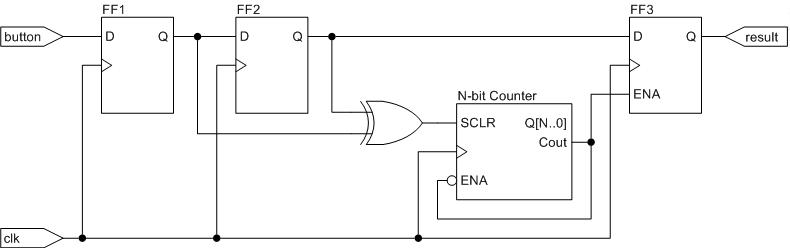
\includegraphics[width=0.7\textwidth]{images/debounce_schematic-from-eewiki.JPG}}
%   \caption{Debouncing circuit example(\href{http://eewiki.net/x/FgBM}{Source : eewiki})}
% \end{figure}
% 
% \subsection{Applying the concepts into VHDL}
% With learning the concepts of debouncing a signal. Next we need to apply the concepts into VHDL. First you will be needing signals to maintain the values of the first two flip flops, the XOR output and a location for the count number. You will need to create a process routine to monitor the clock state. In the process, the flip flops will update their state when there is a \textbf{CLK'event} and with a value of \textbf{1}. This can be translated to a rising action on the clock line. Next you will need to check the flip flop states and reset the count if both flip flops have different states. The output will happen if the most significant bit will turn \textbf{1}. It is recommend reviewing the debounce.vhd source and get a understanding of what is happening.
% 
% \subsection{Building and Flashing the button debouncer project}
% Now is the time to build the seven segment display. First create a new project just like in the counter section. Add the source in the Button folder, there will be three files. Build, and flash it on the Nexys 2 dev board(refer to counter). Don't forget to check the VHDL code and see what is happening.
% 
% \subsection{Button Debouncing Questions}
% 
% \begin{enumerate}
%   \item Demonstrate to the TA or professor the button controller.
%   \item Why would you incorporate a enable in the button controller?
% \end{enumerate}
% 
\newpage

\section{3. VGA Display concepts part 2:}
% In this section, you will be learning how a 7-segment display can be incorporated in VHDL. While observing the Nexys 2 dev board, you will notice that there are four 7-segment displays. These displays can be very useful to use as a debug device since there can be 4 bytes of data displayed.
% 
% \subsection{Reviewing 7-Segment Display}
% Just refresher each 7-segment display is tied to a common cathode while one anode per display. The cathodes are a ground sink while the anode supply the power. For the display you do not want to have the number flicker. So the display should oscillate around 60Hz. Since there are four displays you need to alternate between them. This will give us 240Hz for alternating between each number without flickering.
% 
% \subsection{Applying the concepts into VHDL}
% Inorder to apply this in VHDL, you need to break down the 7-segment driver into resonable chunks. First you will need a clock divider that will change a 50Mhz clock signal into 240Hz. Next you will need a 7-segment decoder, this can be don in a select statement in VHDL. The Last major part is the display driver to cycle between the 7-segment display and output the correct number. Look at the SevenSeg.vhd file to get a grasp of the concept. The top level connects the SevenSeg out to the board and helps provide values for the 7-segment display.
% 
% \subsection{Building and Flashing the 7-segment Display project}
% Create a new project and add the source in the SevenSegment folder. Build the 7-segment display and flash it to the Nexys. Test the Seven Segment display by flipping the dip switches to control the first two displays.
% 
% \subsection{7-Segment Display Questions}
% 
% \begin{enumerate}
%   \item Adjust the VHDL code and the I/O to make the 7-seg display "FACE"
%   \item Demonstrate to the TA or professor the 7-seg display
%   \item What is the clock speed in the 7-segment display driver and why?
% \end{enumerate}
% 
% \begin{figure}[!htb]
%   \centering
%     \fbox{\includegraphics[width=0.5\textwidth]{images/7segFACE.png}}
%   \caption{7-segment Display output FACE}
% \end{figure}
% 
\newpage

\section{4. Debug Unit:}
% In this section of the lab, you will be getting familiar with simulating VHDL in ISE. You are presented a complete source of an ALU. A ALU is a Arithmetic device which will output specific values based on operating codes(opcodes). For the ALU you will have two 8 bit input values(A,B) and a opcode. The output will have the result of the operation plus a condition code register.
% \subsection{Concepts of a ALU}
% In this Lab you will be using an 8-bit ALU. The ALU is a collection of operations. These operations can be add, subtract, AND, OR, Shift and much more. For the ALU you can see what operations it performs based on the opcodes in the table below.
% 
% \begin{table}[!htb]
%   \begin{center}
%     \begin{tabular}{|l|l|l|l|}
%        \hline
%        OPCODE & operation & procedure & CCR\\
%        \hline 
%        0000 & ADDITION & RA \textless = RA + RB & NZVC \\
%        0001 & SUBTRACTION & RA \textless = RA - RB & NZVC \\
%        0010 & AND & RA \textless = RA \& RB & NZVC \\
%        0011 & OR & RA \textless = RA \textbar \enspace RB & NZVC \\
%        0100 & COMPARE & RA \textless = 0, NZ change & NZ \\
%        0101 & ADD Immediate & RA \textless = RA + IMMED & NZVC \\
%        0110 & AND Immediate & RA \textless = RA \& IMMED & NZVC \\
%        0111 & SHIFT LEFT & RA \textless = RA$<<$IMMED & VC \\
%        1000 & SHIFT RIGHT & RA \textless = RA$>>$IMMED  & \\
%        1001 & LOAD WORD & RA \textless = ALU\_MEM  & \\
%        1010 & STORE WORD & ALU\_MEM \textless = RA & \\
%        \hline
%     \end{tabular}
%   \end{center}
%   \caption{ALU OPCODE}
% \end{table}
% 
% \subsection{Setting up a ALU in VHDL}
% Create a new project or use a existing and remove the files. Add all the source files in the ALU folder to the project. In this project you will be using the simulation utility in Xilinx. In order to run a simulation, you will need to create a Behavioral vhd file. This file will simulate the inputs to a VHDL design you are implementing. This will be able to aid in testing your code for and prone errors that may arise during your testing of the code.
% 
% \subsection{Testing the ALU by simulation}
% In order to start simulation you must switch you view from Implementation to Simulation, this can be done by \textbf{Design -\textgreater View -\textgreater Simulation}. When you in simulation mode, select \textbf{ALU\_tb\_vhd}. Under the Design tab you will see ISim Simulation and two operations. Behavioral Check Syntax and Simulate Behavioral Model. Run the Simulate Behavioral Model, there will be a graph poping up with the simulation results from the test bench file.
% 
% \begin{figure}[!htb]
%   \centering
%     \fbox{\includegraphics[width=0.5\textwidth]{images/XilinxSelectSimulation.png}}
%   \caption{Select Simulation Mode in ISE}
% \end{figure}
% 
% \begin{figure}[!htb]
%   \centering
%     \fbox{\includegraphics[width=0.5\textwidth]{images/XilinxStartSimulation.png}}
%   \caption{Start Simulation in ISE}
% \end{figure}
% 
% \newpage
% \subsection{ALU test bench Questions}
% \begin{enumerate}
%   \item Take a screen shot of the simulation from 50ns - 300ns
%   \item Change CCR value at line 110 from \textbf{1010} to \textbf{0000}. Rerun the simulation, what do you notice in the console and why does it happen?
% \end{enumerate}
% 
\newpage

\section{5. Assembling a Keyboard Debug Unit:}
% With each section you learned various concepts and was given code to run. Now it is your turn to create some VHDL code. In the previous sections you learned how to interface with the Nexys board Dip switches, Led's, mechanical buttons, and the seven segment display. You also learned about a ALU. For this section you will be combining them together and creating a user input ALU. The method of input and output is all up to you.
% 
% \subsection{Jumping into VHDL}
% Since this will be your first time coding VHDL for the project. You will have to devise a method for your ALU to interface with. First you need to create a block diagram of each device connected together. After that give more in depth design in a RTL. Build your design in VHDL with a reference of the top\_level designs in the other sections of the lab.
% 
% \subsection{Building, Flashing and testing a user input ALU project}
% This part will take you the most time to accomplish out of all the sections. You will have to debug you code and see how it runs on the Nexys 2 dev board. The building and flashing will always be the same methods in any lab. You will also be needing to create a Acceptance Test Plan(ATP) to validate that your project is working.
% 
% \subsection{Final Questions}
% \begin{enumerate}
%   \item Demonstrate to the TA or professor the user input ALU.
%   \item What was the biggest challenge you overcame?
%   \item If you would rebuild this, how you change it?
%   \item What is your confidence level in VHDL and explain why.
%   \item Any ideas to improve the Lab?
% \end{enumerate}


\newpage

\section{6. Extra 1: Keyboard ALU part 1:}


\newpage

\section{7. Extra 2: Keyboard ALU part 2:}

\newpage

\section{Lab 2 Grade}

\begin{table}[!htb]
  \begin{center}
    \begin{tabular}[width=0.8\textwidth]{|l|l|c|l|}
       \hline
       Section & Description & Value & Score\\
       \hline 
       \multicolumn{2}{|l}{\textbf{Section 1}}  & -\textbf{30}- &\\
       \hline
       1.1. Keyboard Demo & Demonstrate Keyboard Controller & 20 &\\
       1.2. Questions & Answer Questions about the Keyboard Controller & 10 &\\
       \hline
       \multicolumn{2}{|l}{\textbf{Section 2}}  & -\textbf{20}- &\\
       \hline
       2.1. VGA Demo 1 & Demonstrate RGB VGA Display & 10 &\\
       2.2. Questions & Answer Questions about the VGA Display & 10 &\\
       \hline
       \multicolumn{2}{|l}{\textbf{Section 3}}  & -\textbf{10}- &\\
       \hline
       3.1. VGA Demo 2 & Demonstrate VGA Terminal Display & 5 &\\
       3.2. Questions & Answer Questions about the VGA Terminal Display & 5 &\\
       \hline
       \multicolumn{2}{|l}{\textbf{Section 4}}  & -\textbf{10}- &\\
       \hline
       4.1. Debug Unit Demo &  Demonstrate Debug Unit & 5 &\\
       4.2. Questions & Answer Questions about the Debug Unit & 5 &\\
       \hline
       \multicolumn{2}{|l}{\textbf{Section 5}}  & -\textbf{10}- &\\
       \hline
       5.1. VGA Debug Unit & Demonstrate VGA with Debug Unit & 5 &\\
       5.2. Questions & Answer Questions about the VGA Debug Unit & 5 &\\
       \hline
       \multicolumn{2}{|l}{\textbf{Section 6: Extra Credit 1}}  & -\textbf{20}- &\\
       \hline
       6.1. ALU Debug Unit & Demonstrate Debug Unit with ALU & 20 &\\
       \hline
       \multicolumn{2}{|l}{\textbf{Section 7: Extra Credit 2}}  & -\textbf{20}- &\\
       \hline
       7.1. ALU Terminal & Demonstrate ALU with VGA Terminal & 20 &\\
       \hline
       \multicolumn{2}{|l}{\textbf{Lab Report}}  & -\textbf{20}- &\\
       \hline
       \hline
       \multicolumn{2}{|l}{Total} & \multicolumn{1}{c|}{100|140} &\\
       \hline
    \end{tabular}
  \end{center}
  \caption{Lab Grade Breakdown Table}
\end{table}

\end{document}
